\chapter{Discussion}

The \acrshort{ewc} paper is currently one of the most known approaches to overcome catastrophic forgetting.
Their paper shows that it performs well on a permuted MNIST dataset with three sequential learning tasks.
\newline
Unfortunately, the paper just delivers main facts and ideas behind the \acrshort{ewc} solution.
It has a lack of some important facts to understand their approaches and test benchmarks.
They do show the main idea, formula and advanatges by using them.
Nevertheless, they do not explain why they are using the \acrshort{fim}, in fact just the diagonal of the \acrshort{fim}.
Moreover, they do not document helpful formulas, like the \acrshort{fim} or deeper calculation insights.
Even a code base is not available.
In the appendix some parameters of their benchmarks are documented.
Yet, their benchmarks for supervised learning (Figure \ref{fig:ewc_permuted_example}) on the MNIST dataset are not reproducible.
They do not present a solution for a reasonable lambda value, learning rate or iterations for the re-training.
Therefore, own benchmarks had to be created.
The benchmarks refer to the report \cite{cf_application_oriented_study} which includes an application-oriented study on the \acrshort{ewc} algorithm.
The network was given three hidden layers with 800 neurons.
This feature base is a proven structure for the MNIST problem.
The iterations and batch sizes are chosen from the study \cite{cf_application_oriented_study}.
In the permuted benchmark the iterations are increased.
The increase helps to analyze the surpassing of the $T_2$ accuracy to the complete dataset.
Lambda was initialized to $\lambda = \frac{1}{learning \: rate \: T_2}$ by default.

Currently there are multiple implementations of \acrshort{ewc} available.
Most of them are created with PyTorch, a similar open-source machine learning library to Tensorflow.
Still, there are two solutions implemented in Tensorflow and available on GitHub
\footnote[1]{\url{https://github.com/ariseff/overcoming-catastrophic}}
\footnote[2]{\url{https://github.com/stokesj/EWC}}.
Both show a solution for a permuted MNIST on supervised learning but not a disjoint MNIST.
\newline
The more popular implementation\footnotemark[1] modifies the original algorithm.
For the \acrshort{fim} calulation it does not use the given labels from the dataset.
It generates new labels based on a randomization of the softmax probabilities.
% Moreover, the CrossEntropy loss funtion is not properly used for calculating the gradients.
% They avoid to negate the log from CE
\newline
The second implementation \footnotemark[2] is used in the report \cite{cf_application_oriented_study}.
As discovered in Section \ref{project_review_improvements}, it is built with a workaround to be able to perform per-gradient calculations in Tensorflow.
This code base was the inspiration for the default lambda value.
\newline
The reimplementation of \acrshort{ewc} in Python and Tensorflow for this article omits these drawbacks and enables an easy adoption of the \acrlong{gm} (Section \ref{project_review_improvements}).

The baseline shows that the \acrshort{ewc} algorithm works with the three benchmarks.
This \acrshort{ewc} algorithm (Figures \ref{fig:ewc_d9-1}, \ref{fig:ewc_d5-5}, \ref{fig:ewc_p10-10}) shows that it reduces catastrophic forgetting (Figures \ref{fig:catastrophic_forgetting_d91_example}, \ref{fig:catastrophic_forgetting_d55_example}).
However, it does not solve catastrophic forgetting for these benchmarks on the MNIST dataset.
\newline
The application-oriented study \cite{cf_application_oriented_study} discoveres that \acrshort{ewc} is in some way effective against \acrlong{cf} for simple \acrshort{slt}s (D9-1 benchmark), but ineffective against \acrlong{cf} for more complex problems (D5-5 benchmark) \cite{cf_application_oriented_study}.
\newline
In the benchmark D9-1, the complete dataset peaks at 99\% accuracy in the re-training and completes the re-training with 71\% accuracy \cite{cf_application_oriented_study}.
The results in the baseline (Figure \ref{fig:ewc_d9-1}) show a peak of 92\% und an end result of 80\% accuracy.
These statistics are quite similar.
\newline
In the D5-5 benchmark, the application-oriented study can not register any sign of learning.
The study documents a peak of 50\% and 31\% accuracy at the end of the re-training \cite{cf_application_oriented_study}.
In comparison to these results, the baseline in this article (Figure \ref{fig:ewc_d5-5}) shows that there is learning happending.
This benchmark substantiates a peak of 82\% and an end result of 81\%.
\newline
In the reference paper, the third permuted benchmark \cite{cf_application_oriented_study} shows a peak of 100\% and an end result of 98\% after the re-training.
The result of the baseline in Section \ref{project_baseline} (Figure \ref{fig:ewc_p10-10}) is lower with a peak and an end result of 90\%.
\newline
It is important to note, that on one side the covered reimplementation needs to be retrained with a lower learning rate of 0.00001.
On the other side, the training is done with a learning rate of 0.001.

The comparison of $T_2$ in Figure \ref{fig:ewc_d5-5} and $T_1$ in Figure \ref{fig:ewc_p10-10} shows that in the D5-5 benchmark it would be much easier to train a new model with the complete MNIST dataset.
Because of the same iterations, the same batch size and a smaller learning rate of $T_1$ (in Figure \ref{fig:ewc_p10-10}), the perfromance of training the complete dataset instead of retraining with the \acrshort{ewc} algorithm would increase the accuracy.
As proposed in the section catastrophic forgetting (Section \ref{catastrophic_forgetting}), there will be a sacrifice of knowledge by using the \acrshort{ewc} algorithm.
Though, these benchmarks are just a small representation of the problems in a largely scaled environment for models and datasets.
In this case MNIST just provides a simplification of the problem to be able to test an algorithm.
It gives the ability to test several different parameters in a short amount of time and computation power.
So these benchmarks help to get a better understanding of the algorithm.
\newline
Of course, as described in the motivation (Section \ref{intro_motivation}), the goal is to get to an artificial general intelligence, where an algorithm can behave like a human brain.
In order to get there, the algorithm has to be able to work with small datasets like MNIST as well.
But if the main challenges of \acrshort{ewc} are solved and the algorithm is ready for deployment, its first use would be in scenarios where multitask learning (Figure \ref{fig:intro_motivation_multitask_learning_paradigm}) is not an option.
That is, because \acrshort{ewc} only reduces catastrophic forgetting, instead of solving it.

There are multiple ways to implement the \acrshort{ewc} algorithm with Python and Tensorflow.
The attached codebase \footnote{\url{https://github.com/florianwiech/incremental-machine-learning}} tried multiple implementations.
First implementations dealt with own datasets, iterators and network classes.
The advantage is that the developer has full control over the complete code.
Though, a big disadvantage is, that other developers need a lot of effort to understand the code.
This is why developers should use the given helper classes of included frameworks.
Most of the time they present a good documentation and other developers, who know the framework, are able to understand the code quite quickly.
Because of that reason the code was converted to built-in Tensorflow classes like the Dataset, Iterator and autoloading of the MNIST dataset.
This code sticks as close as possible to the Tensorflow provided classes and Low-Level API.
But along the way of converting the code to the Tensorflow classes, the developer of the code just lost a lot of control and the ability to see what exactly being calculated by just looking at the code.
This is a huge disadvantage with the built-in classes of Tensorflow.
\newline
Through the own implementation, the option between a \acrshort{fim} calculation and the \acrshort{gm} matrix is straightforward by adjusting the "batch\_matrix" variable.
Since both computations with a batch size of 1 are the same, the modification is applied when the batch size is higher than one.

The baselines shows the performance of the original EWC algorithm and the experiments test the adaption of the \acrlong{gm}.
In comparison, the benchmarks look encouraging:
\newline
In the \textbf{benchmark type D9-1}, the comparison of the experiment (Figure \ref{fig:exp_d9-1_bs1k}) and the baseline (Figure \ref{fig:ewc_d9-1}) shows that the algorithm does work with the \acrshort{gm}.
The complete dataset in Figure \ref{fig:ewc_d9-1} has a peak of 93\% and an end accuracy of 86\% compared to Figure \ref{fig:exp_d9-1_bs1k} with a peak of 93\% and at the end 85\%.

\begin{figure}[H]
    \centering
    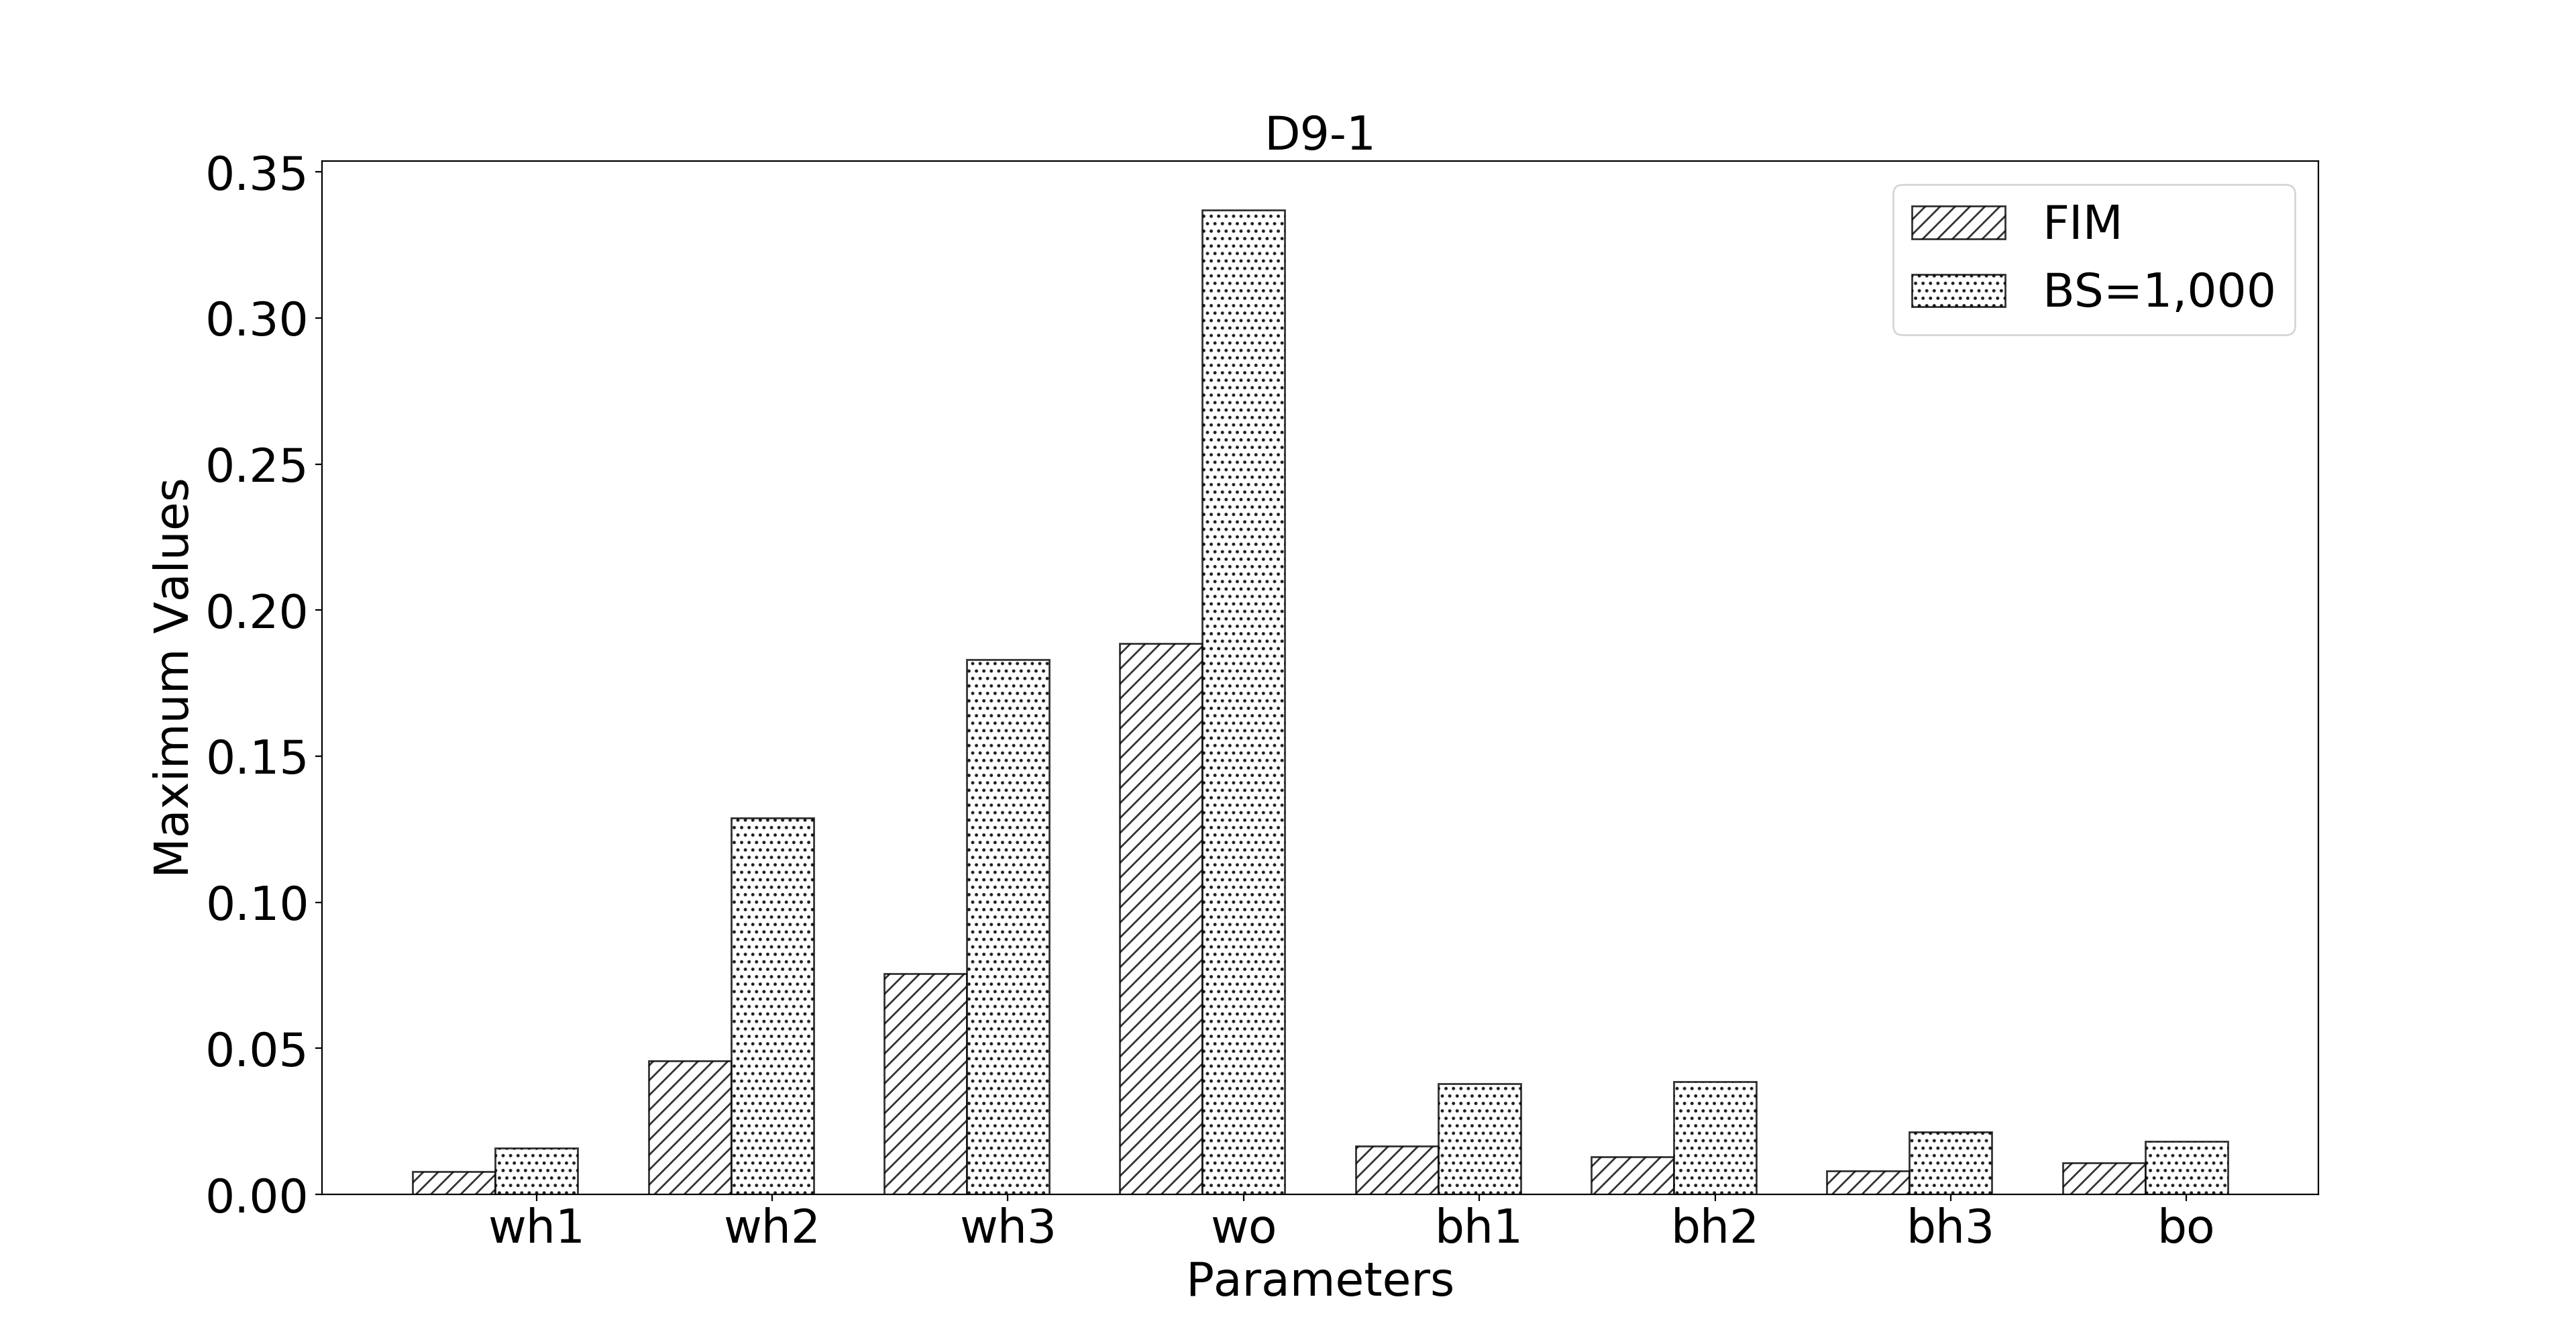
\includegraphics[width=\textwidth]{project/discussion/D91_grad_max}
    \caption{D9-1 Gradients}
    \label{fig:dis_d91}
\end{figure}

To get deeper insights, Figure \ref{fig:dis_d91} shows the maximum calculated gradients of each weight matrix and bias vector after the re-training.
The Parameters represent the set of weights and biases.
It shows only the maximum values, because the minimum values are all approximatively zero.
It is interesting that in this case the maximum gradients of the \acrshort{gm} are often 200\% the size of the \acrshort{fim} gradients.
But the re-training is in both cases similar.

In the \textbf{D5-5 benchmark}, Figure \ref{fig:ewc_d5-5} compared to Figure \ref{fig:exp_d5-5_bs1k} are very similar.
Both benchmarks peak at 82\% accuracy and end up with roughly 80\% accuracy.
This means that both calculations do work.
Still, the \acrshort{gm} takes half of the computation time compared to the original \acrshort{fim} calculation.
This happens, because the \acrshort{fim} computes the square of every gradient.

\begin{figure}[H]
    \centering
    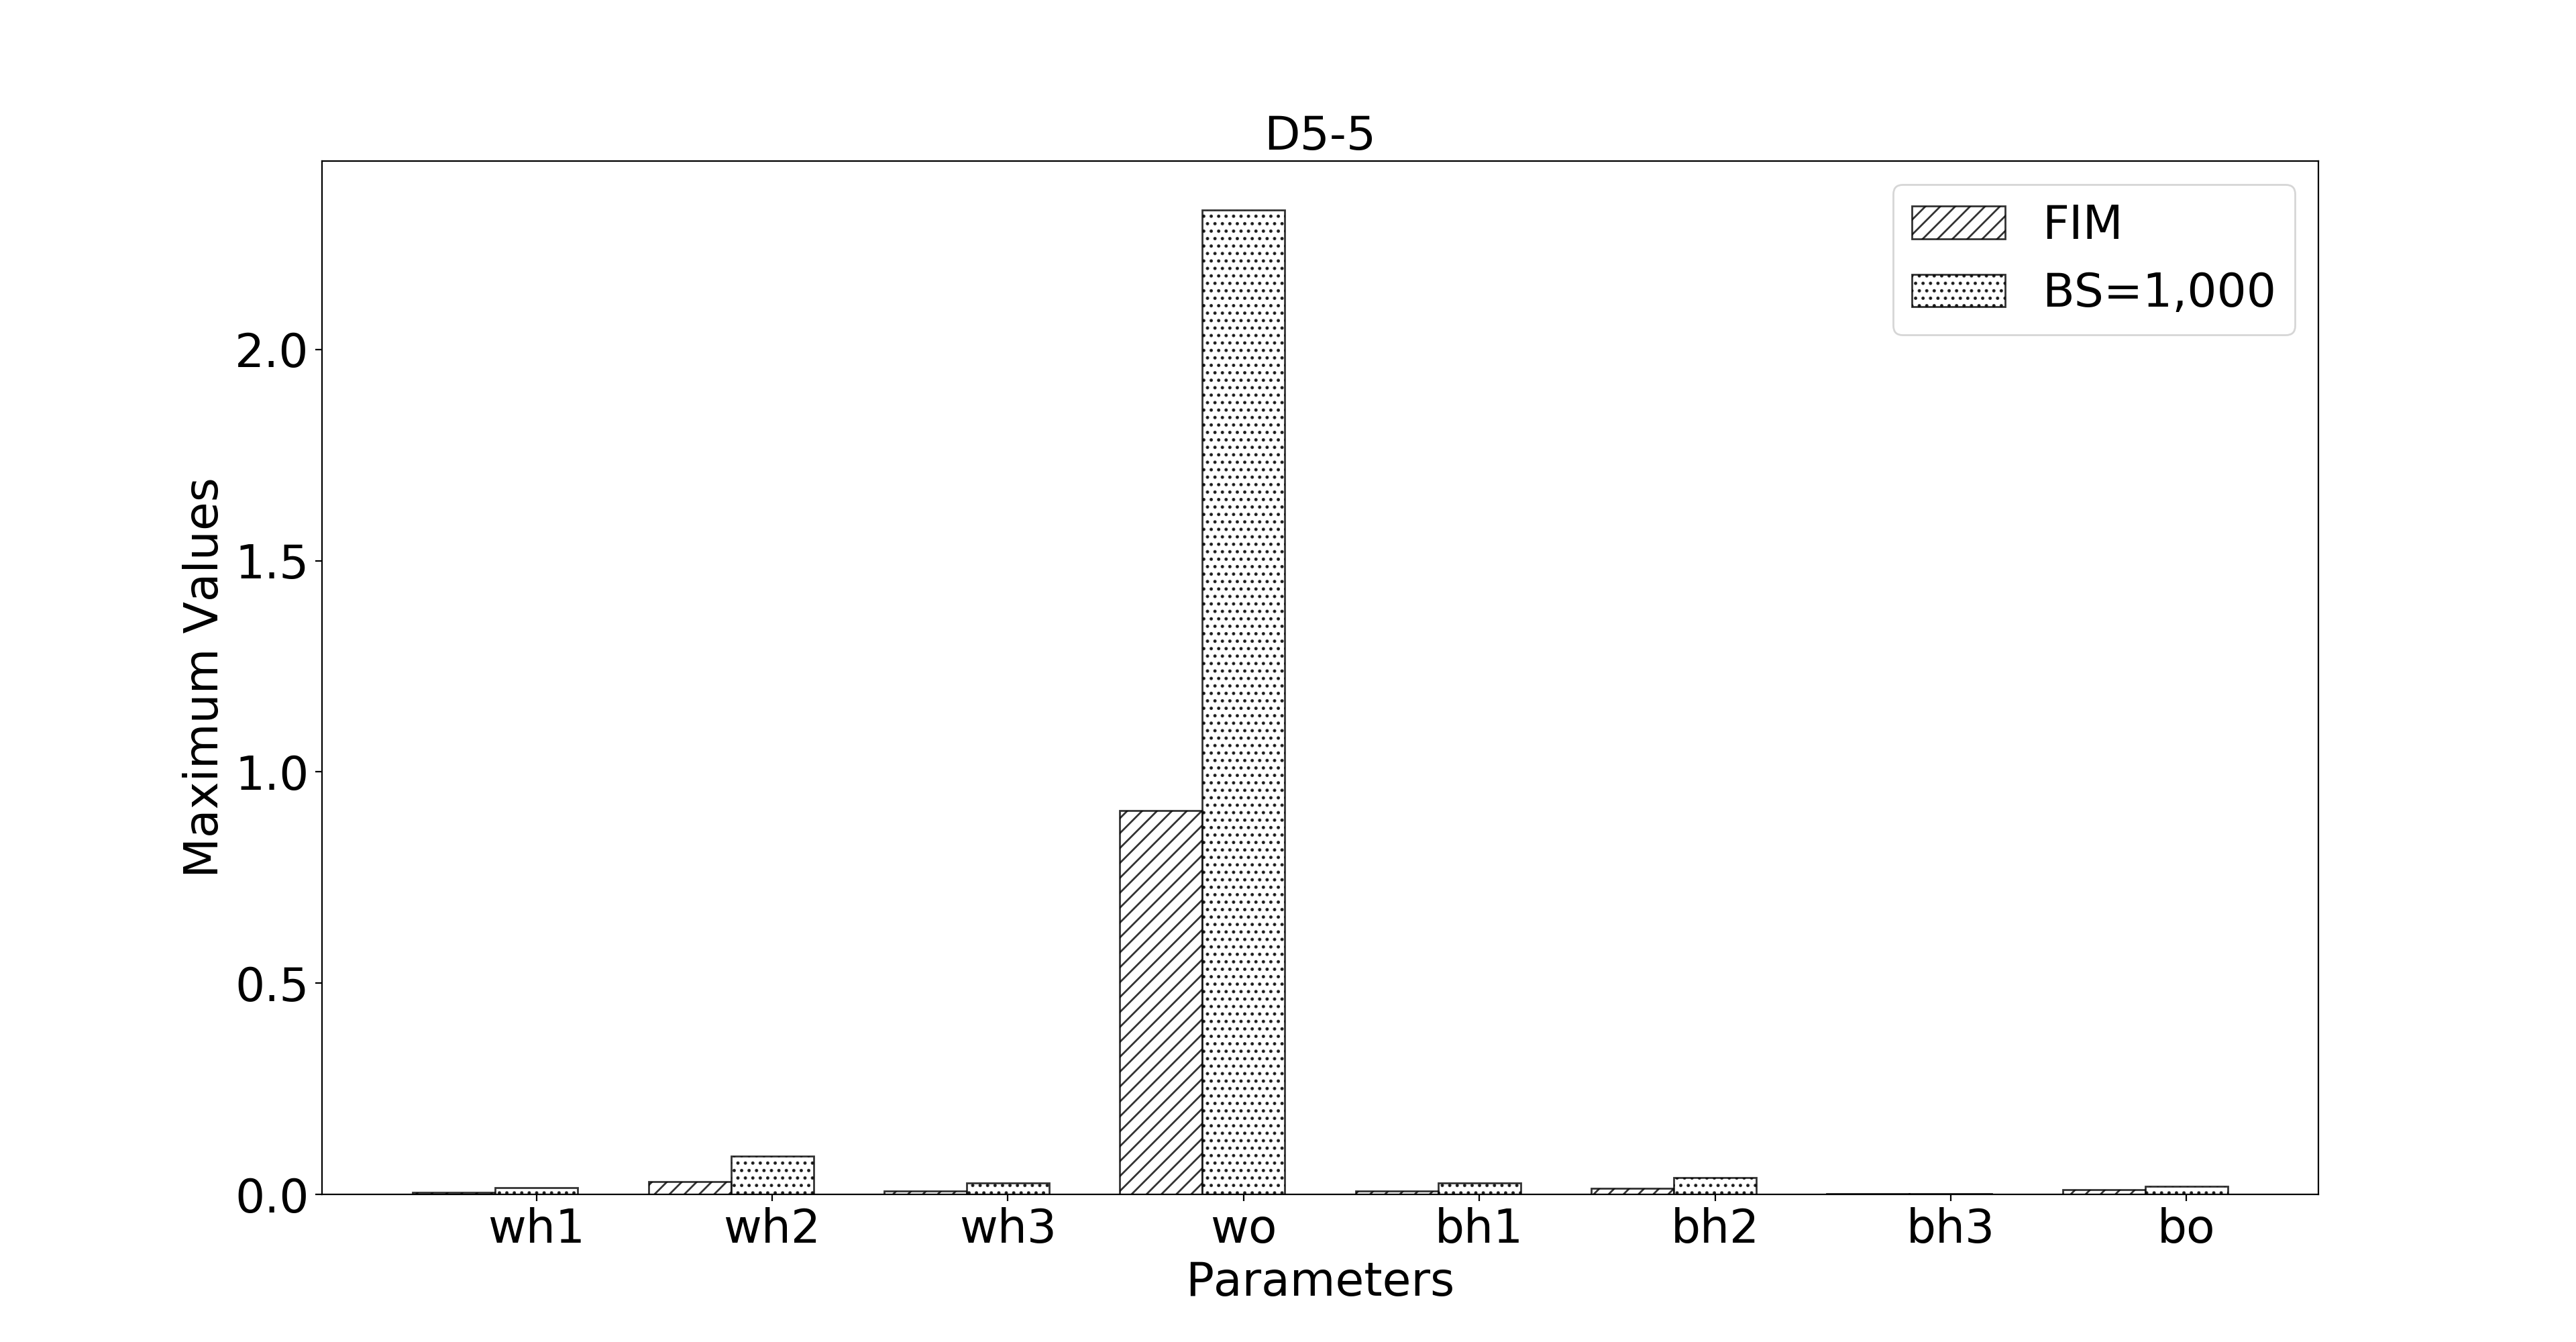
\includegraphics[width=\textwidth]{project/discussion/D55_grad_max}
    \caption{D5-5 Gradients}
    \label{fig:dis_d55}
\end{figure}

Figure \ref{fig:dis_d55} shows a composition of the extrem gradient values.
As well as the D9-1 benchmark, the maximums show differences, yet, they do not differ in the re-training.

These gradient figures of the two benchmarks (Figure \ref{fig:dis_d91}, Figure \ref{fig:dis_d55}) do show differences in the comparison of every value.
Figure \ref{fig:dis_d91} exhibits more variations.
Both \acrshort{gm} matrices were calculated with an training set $N$ of 1,000 samples.
Nervertheless, their complete size of samples and the calculated weights and bias values differs.
The D9-1 benchmarks calculated 54 averaged gradients or 54,000 per-gradients and the D5-5 benachmark 30 averaged gradients or 30,500 per-gradients.

In the \textbf{P10-10 benchmark}, the baseline (Figure \ref{fig:ewc_p10-10}) and the experiment (Figure \ref{fig:exp_p10-10}) show that both re-trainings result in the same accuracy of 90\% on the complete dataset.
\newline
The several parameter tests (Table \ref{table:exp_p10-10}) document, that multiple parameter combinations of learning rate and lambda produce an auspicious result.
The combination of a small learning rate and a small lambda value outperform higher parameter values.

\begin{figure}[H]
    \centering
    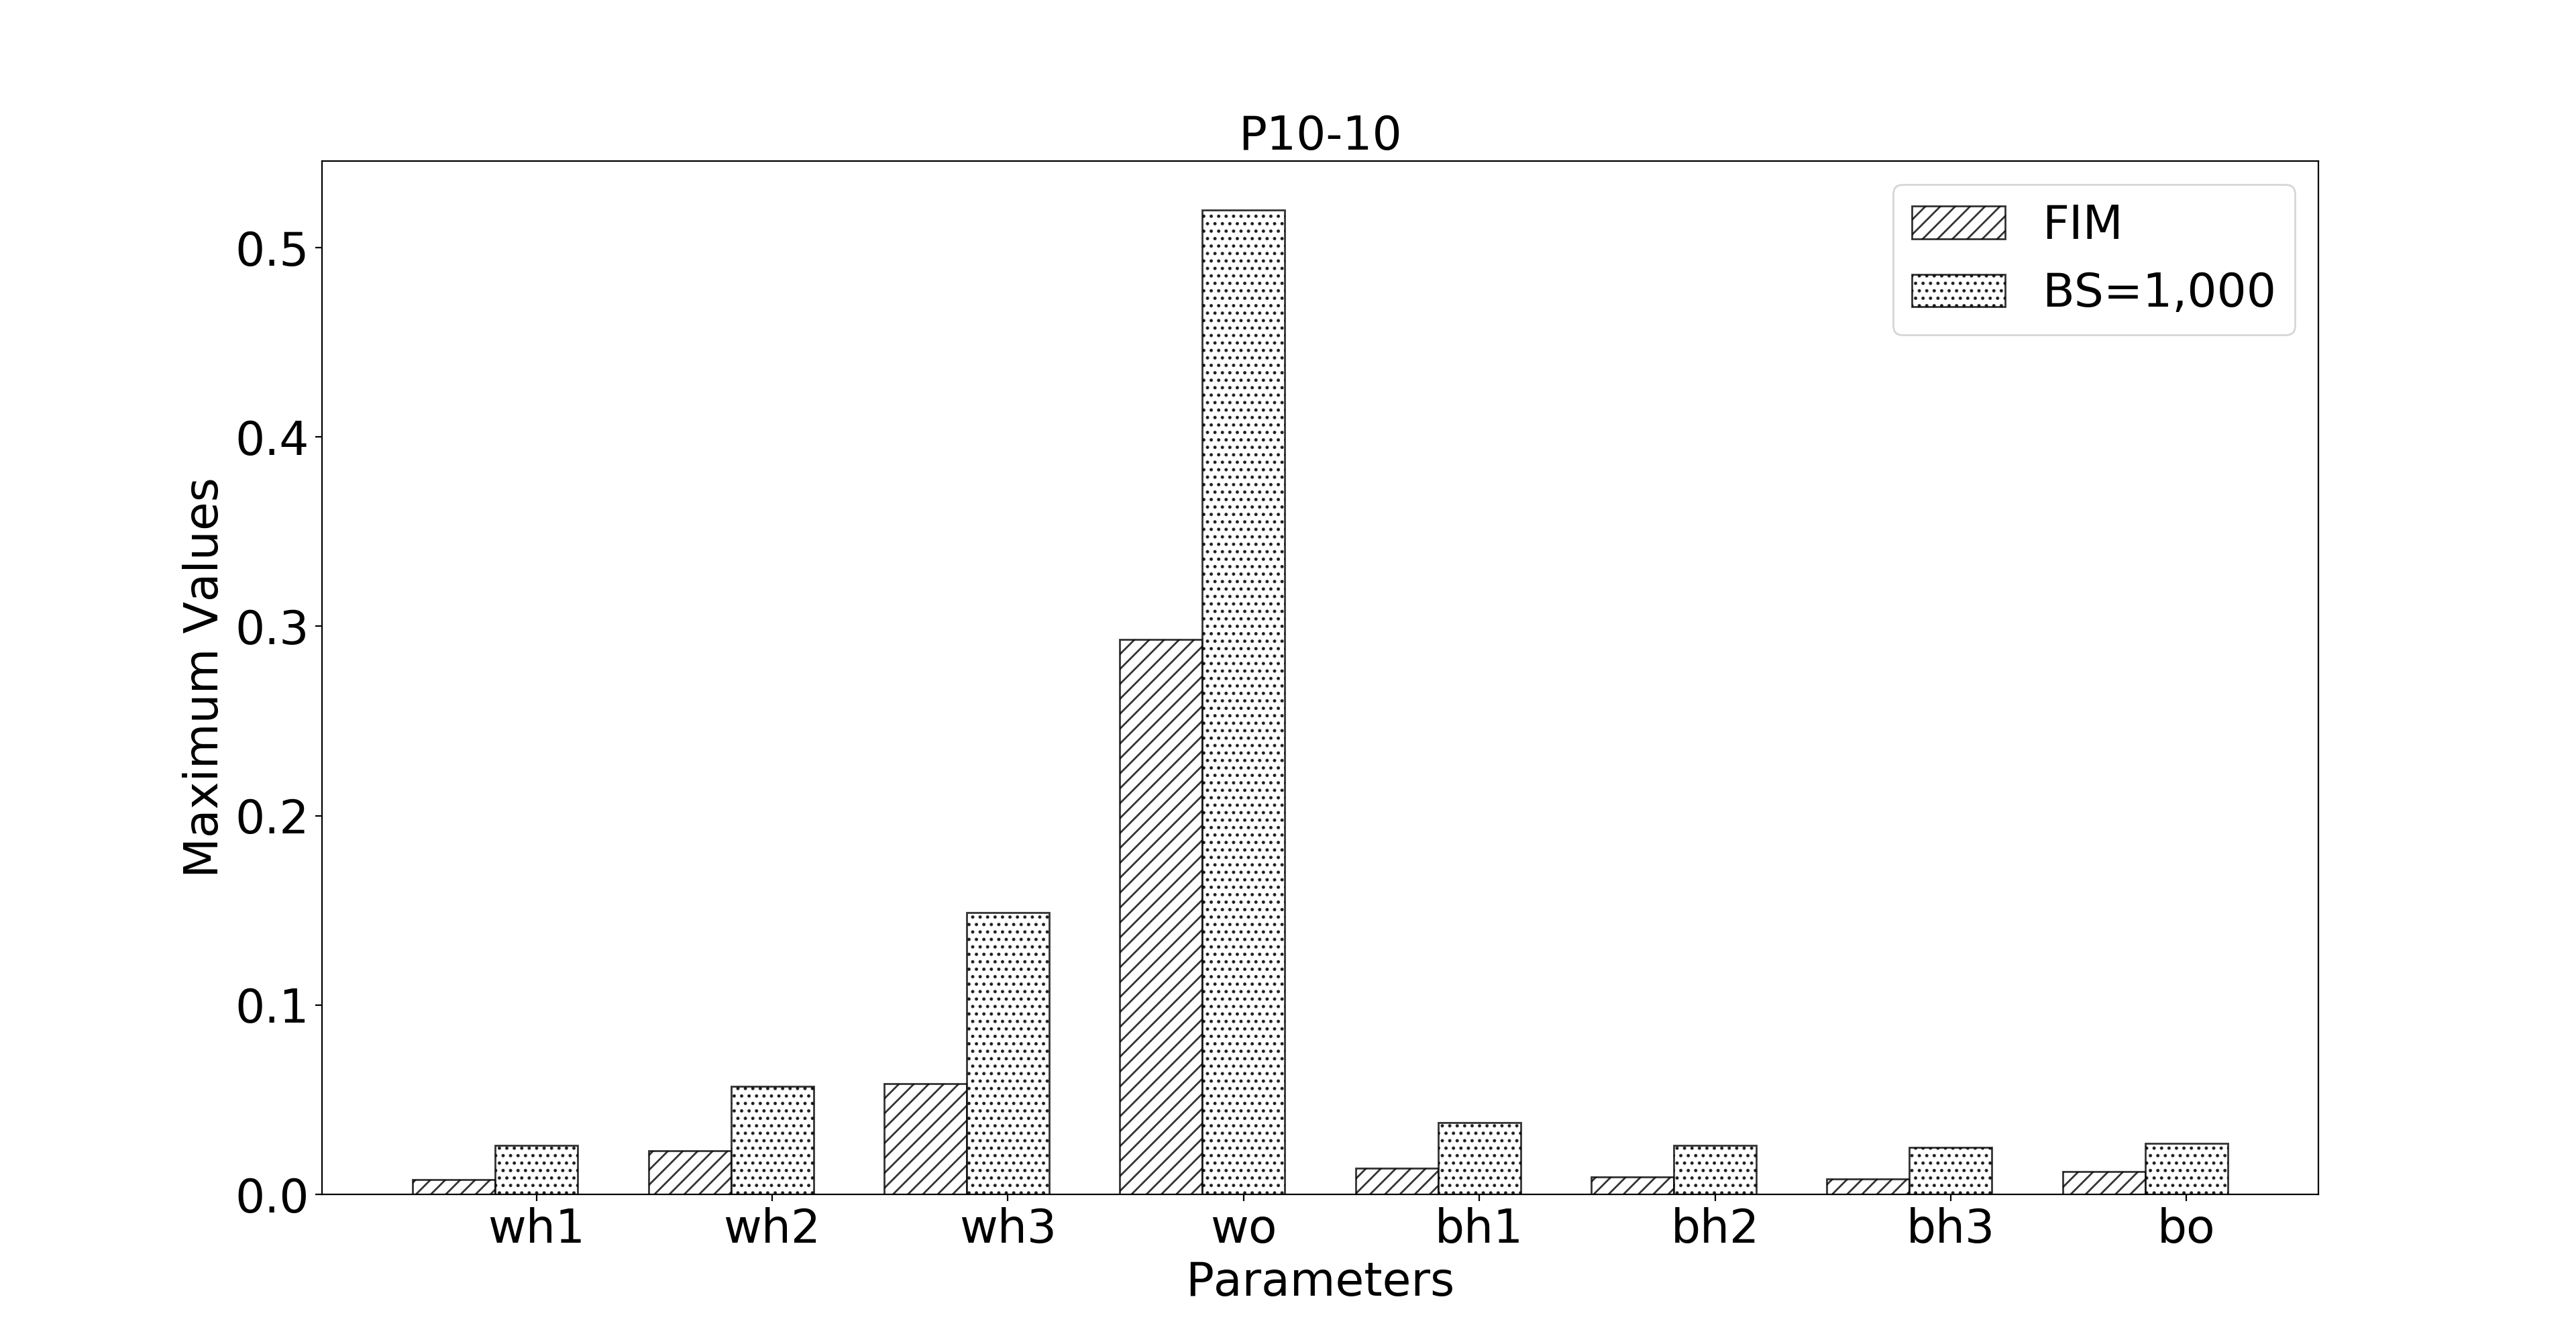
\includegraphics[width=\textwidth]{project/discussion/P1010_grad_max}
    \caption{P10-10 Gradients}
    \label{fig:dis_d1010}
\end{figure}

Figure \ref{fig:dis_d1010} shows the comparison of the gradient maximums.
As well as the other benchmarks, the maximum values of the \acrshort{gm} are much higher than the maximum values of the \acrshort{fim}.

The promising benchmarks in this article worked with fixed iteration counts, learning rates and a default lambda value.
In preparing the three parameters had to be tested with multiple combinations.
Currently there is no solution, how to choose the quantity of iterations, learning rate or the lambda value.
So the developer needs to specify the importance of the \acrshort{ewc} appendix.
The reference implementation set it to $\lambda = \frac{1}{learning_rate \: T_2 }$, but we can clearly see in
the parameter test in the D9-1 (Table \ref{table:exp_d9-1}) and D5-5 (Table \ref{table:exp_d5-5}) benchmarks, that this does not output the best result.
Even the comparison of these tables show, that the chosen values for the best result differ from each other.
Regarding the tables it is important to note, that they just tested the learning rate and lambda value on a fixed iteration count.
But the number of iterations is a important component in the training process and can quickly collide with the other two parameters.
A solution for an iteration count might be the continual execution of a network test after every training step.
With this approach, the network tests its status and can cache promising models.
If the subsequent training steps do not show any better results, the training process can be terminated and the best cached model loaded.
This approach definitly increases the training time and computations.
Although it is able to intercept useless training.
Overall a solution for the parameter choice might not be trivial.
\newline
For now the devleoper has to test multiple parameter combinations in order to find out, if this algorithm presents an useful outcome.
Every new task has to be tested with multiple parameter varations in order to get feedback if there is a promising result.
This is a big problem and makes the algorithm really weak compared to the current multitask learning method.
The \acrshort{ewc} algorithm is not predictible to get any result, but multitask learning will present a result with a measurable period, which makes it the better choice for now.

\section{Conclusion}

The baseline, experiments and discussion show that the introduced Gradient Matrix is a great simplification for the \acrshort{ewc} algorithm.
It delivers very similar results compared to the Fisher information matrix.
Since the Gradient matrix solves an issue with the \acrshort{ewc} algorithm and the Tensorflow framework it is a better alternative.
The computation is decreased and the algorithm alleviates catastrophic forgetting, but does not prevent it.
However, the \acrshort{ewc} algorithm by itself deals with a lot of truble setting correct parameters.
Overall, the lack of knowledge about a promising parameter choice weaks the \acrshort{ewc} algorithm.
Therefore, it is not useable for real-world scenarios.
For deployment, multitask learning (Figure \ref{fig:intro_motivation_multitask_learning_paradigm}) is the tool of choice for now.

\section{Outlook}

The solution to the EWC hyperparameter problem requires additional research.
Further investigations should exhibit, how many re-trainings are possible, until the model looses its previous acquired knowledge completely.
\newline
The authors of the paper "Keep and Learn: …" \cite{Keep_and_Learn} focus with their algorithms on multi-center single-task learning.
This method seems to be similar to the permuted benchmark shown in this article.
Since, the EWC algorithms performs really good on this benchmark, further research could draw a comparison.
\newline
The introduced Gradient matrix should be investigated with different neural network types, several popular datasets and in other continual learning algorithms.
The related work section (Section \ref{intro_related_work}) present several algorithms.
The \acrshort{imm} and \acrshort{ngd} algorithms use the Fisher information matrix as well.
The integration of the Gradient matrix into these algorithms leads to more analyses.
